


\secnum{1}{Устойчивость}
% 1, 2
\sbsnum{1}{Устойчивость в принципе}
% Понятие об устойчивости, неустойчивости и асимптотической устойчивости движения. Формулировка теоремы Ляпунова об устойчивости по первому приближению для установившихся движений. Критерий Рауса-Гурвица. Понятие о критических случаях в теории устойчивости.

\subsubsection*{Возмущенное движение}
что-то

% \subsubsection*{Функции Ляпунова} %x
% Для простоты будем изучать толко установившиеся движения.
В уравнениях возмущенного движения \eqref{231_5} функции $X_i$ будем считать непрерывными в области
\begin{equation}
	|x_i| < H(= \сonst) \ (i = 1,2,\ldots,m),
	\label{232_9}
\end{equation}
и такими, что уравнения \eqref{231_5} при начальных значениях $x_{i0}$ из области \eqref{232_9} допускают единственное решение.

\begin{to_def}[Функция Ляпунова]
	В области $|x_i| < h$, где $h>0$ --- достаточно малое число, будем рассматривать функции \textit{Ляпунова} $V(x_1, x_2, \ldots, x_m)$, предполагая их непрерывно дифференцируемыми, однозначными и обращающимися в нуль в начале координат $x_1 = x_2= \ldots = x_m = 0$.
\end{to_def}
\begin{to_def}
	\textit{Производной} $d V/ d t$ функции $V$ в силу уравнений возмущенного движения \eqref{231_5} называется:
	\begin{equation*}
	 	\frac{d V}{d t} = \sum_{i = 1}^m \frac{\partial V}{\partial x^i} X_i.
	 \end{equation*} 
	 Таким образом производная от функции Ляпунова также $g(x_1,x_2, \ldots, x_m)$, будет непрерывной в той же облачи и обращаться в нуль в начале координат.
\end{to_def}

\begin{to_def}
	$V(x_1, x_2, \ldots, x_m)$ назовём \textit{определенно-положительной} в области $|x_i|<h$, если всюду в этой облачи, кроме начал координат верно: $V >0$.
	Аналогично с определенной отрицательно. В обоих случаях функция $V$ называется \textit{знакоопределенной}.
\end{to_def}

\begin{to_def}
	Если в области $x_i < h$ функция $V$ может принимать значения только одного знака, но может обращаться в нуль не толко в начале координат, то она называется \textit{знакопостоянной}.
\end{to_def}

\begin{to_def}
	Наконец, если функция может принимать в области как значения большие нуля, так и меньшие, она называется \textit{знакопеременной}. 
\end{to_def}

% \subsubsection*{Основные теоремы прямого метода Ляпунова} %x
% % \subsubsection*{Теорема Ляпунова об устойчивости движения}


Здесь и далее для простоты рассматриваем установившееся движение.

\begin{to_thr}[Теорема Ляпунова об устойчивости]
    Если дифференциальные уравнения возмущенного движения таковы, что существует знакоопределенная функция $V$, производная которой $\dot{V}$ в силу этих уравнений является знакопостоянной функцией противоположного знака с $V$, или тождественно равной нулю, то \red{невозмущенное движение} устойчиво.
\end{to_thr}










% \begin{to_thr}[Теорема Ляпунова об асимптотической устойчивости]
    Если дифференциальные уравнения возмущенного движения таковы, что существует знакоопределенная функция $V(x_1, x_2, \ldots, x_m)$, производная которой $\dot{V}$ в силу этих уравнений есть знакоопределенная функция противоположного знака с $V$, то невозмущенное движение асимптотически устойчиво.
\end{to_thr}



% \subsubsection*{Теоремы о неустойчивости}

\begin{to_def}
    Окрестностью положения равновесия, считая, что положение равновесия находится в точке $q^1=\ldots=q^n=0$, назовём область такую, что
    \begin{equation*}
        |q^i| < h, \hspace{1 cm} (i=1, 2,\ldots,m).
    \end{equation*}
\end{to_def}

\begin{to_def}
    Областью $V > 0$ назовём какую-либо область окрестности положения равновесия, в которой $V(x_1, x_2, \ldots, x_m) > 0$. Поверхность $V = 0$ назовём границей области $V >0$.
\end{to_def}

\begin{to_thr}[Теорема Читаева о неустойчивости]
    Если дифференциальные уравнения возмущенного движения таковы, что существует функция $V(x_1, \ldots, x_m)$ такая, что в сколь угодно малой окрестности положения равновесия существует область $V > 0$ и во всех точках области $V > 0$ производная $\dot{V}$ в силу уравнений принимает положительные значения, \textbf{то} невозмущенное движение неустойчиво.
\end{to_thr}

\begin{to_def}
    Функцию $V$, удовлетворяющую теореме Читаева о неустойчивости, называют \textit{функцией} \textit{Читаева}.
\end{to_def}



\begin{to_thr}[I теорема Ляпунова о неустойчивости движения]
    Если дифференциальные уравнения возмущенного движения таковы, что существует функция $V(x_1, \ldots, x_m)$ такая, что ее производная $\dot{V}$ в силу этих уравнений есть функция знакоопределенная, сама функция $V$ не является знакопостоянной, противоположного с $\dot{V}$ знака, то невозмущенное движенние неустойчиво.
\end{to_thr}

\begin{to_thr}[II теорема Ляпунова о неустойчивости движения]
    Если дифференциальные уравнения возмущенного движения таковы, что существует функция $V$ такая, что её производная, в силу этих уравнений, в области положения равновесия может быть представлена в виде
    \begin{equation*}
        \dot{V} = \textnormal{\ae} V + W,
    \end{equation*}
    где \textnormal{\ae} -- положтельная постоянная, а $W$ \textbf{или} тождественно обращается в нуль, \textbf{или} представляет собой знакопостоянную функцию. Если $W$ -- знакопостоянная функция, а $V$ \textbf{не является}  знакопостоянной функцией: $W V < 0$, \textbf{то} невозмущенное движение неустойчиво (ну и если $w \equiv 0$).
\end{to_thr}

\subsubsection*{Усточивость по первому приближению (I)}
Запишем уравнения установившегося возмущенного движения в виде
\begin{equation}
	\frac{d \vc{x}}{d t} = A \vc{x} + \vc{X}(\vc{x}).
	\label{236_1}
\end{equation}
Функции $X_i$ будем считать аналитическими в окрестности начала координат, причем их разложения в ряды начинаются с членов не ниже второго порядка малости относительно $x_1, x_2, \ldots, x_m$.

Вопрос об устойчивости движения очень часто исследуется при помощи уравнений первого приближения:
\begin{equation}
	\frac{d \vc{x}}{d t} = A \vc{x},
	\label{236_2}
\end{equation}
которые получаются из полных уравнений возмущенного движения \eqref{236_1} при отбрасывании в последних нелинейных относительно $x_1, x_2, \ldots, x_m$ членов.

Можно составить характеристическое уравнение
\begin{equation}
	\det(A - \lambda E) = 0,
	\label{236_3}
\end{equation}
которое в общем виде даст решение $\vc{x} = \sum_{j=1}^m c_j \vc{j}_j e^{\lambda_j t}$ (плюс квазимногочлены, но опустим).


Однако как правило уравнения возмущенного движения нелинейны. Поэтому возникает задача об определении условий, при которых выводы об устойчивости, полученные из анализа уравнений первого приближения \eqref{236_2}, справедливы и для полных уравнений возмущенного движения \eqref{236_1} при любых нелинейных членах $X_i$. Эта задача была полностью решена Ляпуновым.

\subsubsection*{Устойчивость по первому приближению (II)}
\begin{to_thr}
	Пусть $\lambda_i$ -- корни уравнения $\det(A - \lambda E) = 0$:
	\begin{itemize*}
		\item[1.] Если $\forall \lambda_i$ $\Re \lambda_i < 0$, то невозмущенное движение асимптотически устойчиво независимо от нелинейных членов.
		% $\frac{d \smallvc{x}}{d t} = A \vc{x} + \vc{X}(\vc{x}).$. 
		\item[2.] Если же $\exists \lambda_i \colon  \Re \lambda_i >0$, то возмущенное движение неустойчиво -- тоже независимо от нелинейных членов. 
		\item[3.] Если же $\exists \lambda_i \colon  \Re \lambda_i = 0$, то подбирая нелинейные члены можно показать, что положение как устойчиво, так и неустойчиво.
	\end{itemize*}
\end{to_thr}

\red{Здесь появится доказательство.}

\subsubsection*{Критерий Рауса-Гурвица}
Запишем уравнение \eqref{236_3} в виде
\begin{equation}
	a_0 \lambda^m + a_1 \lambda^{m-1} + \ldots + a_{m-1}\lambda + a_m = 0.
	\label{238_14}
\end{equation}
Коэффициенты $a_0, a_1,\ldots,a_m$ этого уравнения --- вещественные числа. Без ограничения общности $a_0 >0$.

По теореме Виета имеем:
\begin{gather*}
	\frac{a_1}{a_0} = - (\lambda_1 + \lambda_2 + \ldots + \lambda_m),\\
	\frac{a_2}{a_0} = \lambda_1 \lambda_2 + \ldots + \lambda_{m-1} \lambda_m,\\
	\vdots\\
	\frac{a_m}{a_0} = (-1)^m \lambda_1 \lambda_2 \ldots \lambda_m.
\end{gather*}
Таким образом для отрицательности всех вещественных частей корней $\lambda_1, \lambda_2, \ldots, \lambda_m$ необходимо чтобы все его коэффициенты были положительны.

Однако такого утверждения не достаточно. Необходимое и достаточное условие дается критерием Рауса-Гурвица.

\begin{to_def}
	Назовем \textit{матрицей Гурвица}:
	\begin{equation*}
		\begin{pmatrix}
		    a_1 & a_3 & a_5 & \ldots & 0 \\
		    a_0 & a_2 & a_4 & \ldots & 0 \\
		    0 & a_1 & a_3 & \ldots & 0 \\
		    0 & a_0 & a_2 & \ldots & 0 \\
		    \vdots &  & & \ddots & \\
		    & & & & a_m
		\end{pmatrix}
	\end{equation*} 
	% Рекомендуем читателям самостоятельно разобраться в правилах её построения (мнемонических и нет).
\end{to_def}

Рассмотрим главные миноры матрицы Гурвица (\textit{определители Гурвица}):
\begin{equation*}
	\Delta_1 = a_1, 
	\ 
	\Delta_2 = \begin{vmatrix} a_1& a_3\\ a_0&a_2\end{vmatrix},
	\
	\Delta_3 = \begin{vmatrix}
	    a_1 & a_3 & a_5 \\
	    a_0 & a_2 & a_4 \\
	    0 & a_1 & a_3 \\
	\end{vmatrix},
	\ \ldots \ 
	\Delta_m = a_m \Delta_{m-1}.
\end{equation*}

\begin{to_thr}[Критерий Рауса-Гурвица]
	Для того, чтобы все корни характерестического уравнения с вещественными коэффициентами и положительным старшим $a_0$ имели отрицательные вещественные части, необходимо и достаточно, чтобы выполнялись неравенства:
	\begin{equation}
		\Delta_1 >0,
		\
		\Delta_2 > 0,
		\ \ldots \ 
		\Delta_m >0.
	\end{equation}
	Если же хотя бы одно из неравенств имеет противоположный смысл, то характерестическое уравнение имеет корни, вещественные части которых положительны.
\end{to_thr}

% \subsubsection*{Влиянение диссипативных и гироскопических сил на устойчивость равновесия консервативной системы} %x
% 

\begin{to_thr}[Теорема Томсона-Тэта-Четаева]
    Если в некотором изолированном положении равновесия потенциальная энергия имеет строгий локальный минимум, то при добавлении гироскопических и диссипативных сил с полной диссипацией это положение равновесия становится асимптотически устойчивым.
\end{to_thr}
















% \subsubsection*{Влияние гироскопических и диссипативных сил на
неустойчивое равновесие}

Разложим до квадратичных членов кинетическую и потенциальную энергию системы, и приведем к каноническому виду
\begin{equation*}
    T = \frac{1}{2}\sum_{i=1}^n \dot{\theta}_i^2,
    \hspace{1 cm}
    \Pi = \frac{1}{2} \sum_{i=1}^{n} \lambda_i \theta_i^2.
\end{equation*}
Если $\Pi$ положительно определена, то все величины $\lambda_i$ положительны, и положение устойчиво. Если же присутствуют отрицательные $\lambda_i$, то положение равновесия неустойчиво (\red{по теореме о неустойчивости по первому приближению}). 

\begin{to_def}
    Величины $\lambda_i$ Пуанкаре предложил называть \textit{коэффициентами устойчивости}. Число отрицательных коэффициентов устойчивости называется \textit{степенью неустойчивости}. 
\end{to_def}


\begin{to_thr}[]
    \textbf{Если} среди коэффициентов устойчивости хотя бы один является отрицательным, \textbf{то} изолированное положение равновесия не может быть стабилизировано диссипативными силами с полной диссипацией.
\end{to_thr}

\begin{to_thr}[]
    \textbf{Если} степень неустойчивости изолированного положения равновесия консервативной системы нечетна, \textbf{то} стабилизация его добавлением гироскопических сил невозможна. \textbf{Если} степень неустойчивости четна, \textbf{то} гироскопическая стабилизация возможна.
\end{to_thr}

\begin{to_thr}[]
    \textbf{Если} изолированное положение равновесия консервативной системы имеет отличную от нуля степень неустойчивости, \textbf{то} оно остается неустойчивым при добавлении гироскопических сил и диссипативных сил с полной диссипацией.
\end{to_thr}

\begin{to_def}
    Устойчивость, существующую при одних потенциальных силах, называют \textit{вековой}, а устойчивость, полученную с помощью гироскопических сил, -- \textit{временной}.
\end{to_def}


\sbsnum{2}{Устойчивость консервативной системы  (thr Лагранжа, thr Ляпунова)}
% Теорема Лагранжа об устойчивости положения равновесия консервативной системы. Теоремы Ляпунова об обращении теоремы Лагранжа.

% \subsubsection*{Теорема Лагранжа об устойчивости положения равновесия}
% \subsubsection*{Устойчивость равновесия}


\green{
\begin{to_thr}[Общее уравнение статики\footnote{
    Если с необходимостью всё понятно, то достаточность \red{может быть доказана через уравнения Аппеля (см. п. 158, Маркеев П. А.)}.
}]
    Чтобы некоторое допускаемое идеальными удерживающими связями состояние равновесия системы было состоянием равновесия на интервале $t_0 \leq t \leq t_1$, необходимо и достаточно, чтобы для любого момента времени из этого интервала элементарная работа активных сил на любом виртуальном перемещении равнялась нулю, т.е. чтобы выполнялось
    \begin{equation*}
         \sum_{\nu=1}^N \vc{F}_\nu \cdot \delta \vc{r}_\nu = 0 
         \hspace{1cm}
         (t_0 \leq t \leq t_1).
     \end{equation*} 
     Если система является потенциальной, то уравнения примут вид
     \begin{equation*}
         Q_i = - \frac{\partial \Pi}{\partial q^i} = 0.
     \end{equation*}
\end{to_thr}
}

\begin{to_def} 
    Положение равновесия $q=0$ -- \textit{устойчиво по Ляпунову}, если $\forall \varepsilon > 0 \ \ \exists \delta > 0$, такая что 
\begin{equation}
    \forall \ \ |q(t_0)|<\delta, \ |\dot{q}(t_0)|<\delta \colon
    \hspace{0.5cm} 
    |q(t)|<\varepsilon, \ |\dot{q}(t)| < \varepsilon, \hspace{0.5cm} \forall t \geq t_0.
\end{equation}
\end{to_def}

\begin{to_def} 
    Положение равновесия $q=0$ -- \textit{неустойчиво по Ляпунову}, если $\exists \varepsilon > 0 \ \ \forall \delta > 0$, такая что 
\begin{equation}
    \forall \delta > 0 \ \  \exists |q(t_0)| < \delta, \
    |\dot{q}(t_0)| < \delta, \ \ t^* \colon \hspace{0.5cm} 
    |q(t^*)| > \varepsilon \text{ или } |\dot{q}(t^*)| > \varepsilon.
\end{equation}
\end{to_def}























 %x
\subsubsection*{Теорема Лагранжа}

\begin{to_thr}[Теорема Лагранжа-Дирихле]
     Если в положении равновесия конесервативной системы $\Pi(q)$ имеет строгий локальный минимум, то это положение равновесия устойчиво.
\end{to_thr}

\begin{to_lem} 
    При наличии гироскопических и диссипативных сил положение равновесия сохранится. 
\end{to_lem}




\subsubsection*{Теоремы Ляпунова о неустойчивости положения равновесия консервативной системы}


\begin{to_thr}[Теорема Ляпунова о неустойчивости I]
    Если в положении равновесия $\Pi(q)$ не имеет минимума и это определяется по квадратичной форме её разложения в ряд (в окрестности положения равновесия), то это положение равновесия неустойчиво.     
\end{to_thr}


\begin{to_thr}[Теорема Ляпунова о неустойчивости II]
    Если в положении равновесия $\Pi(q)$  имеет строгий максимум и это определяется по наинизшей степени её разложения в ряд (в окрестности положения равновесия), то это положение равновесия неустойчиво.     
\end{to_thr}













\secnum{2}{Нормальные колебания}
% 3, 4

\sbsnum{3}{Малые колебания консервативной системы}
Запишем уравнения Лагранжа для консервативной голономной системе:
\begin{equation*}
    \frac{d }{d t} \frac{\partial L}{\partial \dot{q}} - \frac{\partial L}{\partial q} = 0,
    \hspace{1 cm}
    q \in  M^n;
    \hspace{1 cm}
    q, \dot{q} \in T M^n.
\end{equation*}
Тогда можно сказать, что
\begin{equation*}
    L(q, \dot{q}, t) \colon TM^n \times \mathbb{R}^1 \mapsto \mathbb{R}^1.
\end{equation*}
Параллельным переносом выберем $q=0$ -- положение равновесия. Тогда считаем, что $q(t), \ \dot{q}(t) \in \varepsilon$ -- окрестности. В идеале мы хотим всё линеаризовать, тогда 
\begin{equation*}
    T = T_2 + T_1 + T_0 = T_2 = \frac{1}{2} \dot{q}^i \dot{q}^j A_{ij} (q) \approx \frac{1}{2} \dot{q}\T A(0) \dot{q} + \ldots,
    \hspace{1 cm}
    A(0) = \frac{\partial^2 T(0)}{\partial \dot{q}\T \partial \dot{q}}.
\end{equation*}
 т. к. для консервативных систем $T_1 = T_0 = 0$. 

Аналогично можем сделать для потенциальной энергии
\begin{equation*}
    \Pi = \Pi (0) + \frac{\partial \Pi(0)}{\partial q\T} q 
    + \frac{1}{2} q\T \frac{\partial^2 \Pi (0)}{\partial q\T \partial q} q + \ldots
    \approx \frac{1}{2} q\T C(0) q,
    \hspace{1 cm}
    C(0) = \frac{\partial^2 \Pi(0)}{\partial q\T \partial q}.
\end{equation*}
Таким образом мы пришли к уравнениям вида
\begin{equation*}
    \frac{d }{d t} \frac{\partial T}{\partial \dot{q}} - \frac{\partial T}{\partial q} = - \frac{\partial \Pi}{\partial q} 
    \hspace{1 cm} \Rightarrow \hspace{1 cm}
    \boxed{
    A \ddot{q} + C q = 0.
    }
\end{equation*}
Последнее уравнение называется \textit{уравнением малых колебаний}. Важно, что $A$ -- положительно определена,  в силу невырожденности уравнений на $\ddot{q}$ уравнений Лагранжа.

Из линейной алгебры понятно, что существуют координаты $\vc{\theta} \in M^n$, а также невырожденная матрица перехода к новым координатам $U \colon \vc{q} = U \vc{\theta}$, и $U\T A U = E, \ U\T C U = \Lambda$ -- диагональная матрица. Тогда верно, что
\begin{equation*}
    T = \frac{1}{2} \dot{\vc{q}} A \dot{\vc{q}} = \frac{1}{2} \dot{\vc{\theta}}\T U\T A U \dot{\vc{\theta}} = 
    \frac{1}{2} \sum_{i=1}^{n} \dot{\theta}_i^2.
\end{equation*}
Аналогично для потенциальной энергии
\begin{equation*}
    \Pi = \frac{1}{2} \vc{q}\T C q = \frac{1}{2} \vc{\theta}\T U\T C U \vc{\theta} 
    = \frac{1}{2} \vc{\theta}\T \Lambda \vc{\theta}
    = \frac{1}{2} \sum_{i=1}^{n} \lambda _i \theta_i^2
    .
\end{equation*}
Это ещё сильнее упрощает уравнения Лагранжа:
\begin{equation*}
    A \ddot{\vc{q}} + C \vc{q} = 0
    \hspace{1 cm} \to \hspace{1 cm}
    \ddot{\theta}_i + \lambda_i \theta_i = 0, 
    \hspace{0.5 cm}
    i = 1, \ldots, n.
\end{equation*}
Здесь $\lambda_i$ -- действительные диагональные элементы $\Lambda$. При различных $\lambda$ получаем, что
\begin{align*}
    \lambda_i > 0 
    \hspace{1 cm} \Rightarrow \hspace{1 cm}
    & \theta_i = c_i \sin (\sqrt{\lambda_i} t + \alpha_i); \\
    \lambda_i = 0 
    \hspace{1 cm} \Rightarrow \hspace{1 cm}
    & \theta_i = c_i t + \alpha_i.; \\
    \lambda_i < 0 
    \hspace{1 cm} \Rightarrow \hspace{1 cm}
    & \theta_i = c_i \exp( \sqrt{-\lambda_i} t) + \alpha_i \exp(-  \sqrt{-\lambda_i} t). \\
\end{align*}
где последние два -- уже не  колебаниям.


Возвращаясь к удобной форме, получаем, что
\begin{equation*}
    \vc{q} = U \vc{\theta} = \sum_{i=1}^{n} c_i \vc{u}_i \sin (\sqrt{\lambda_i} t + \alpha_i),
\end{equation*}
где $\vc{u}_i$ -- амплитудный вектор $i$-го главного колебания.
\texttt{Таким образом консервативная система движется по суперпозиции некоторых главных колебаний (гармонических осцилляций).} 

Иначе мы можем интерпретировать это так, что кинетическая энергия\footnote{
    Переписать грамотнее.
} образует некоторую метрику, а амплитудные вектора образуют некоторый ортонормированный базис.
\begin{equation*}
    U\T A U = E
    \hspace{0.5cm} \Rightarrow \hspace{0.5cm}
    \vc{u}\T_i A \vc{u}_j = \delta_{ij}
\end{equation*}


% \subsection{Решение задач}

Получив матрицы $A, \ C$ переходим к $[C - \lambda A] \vc{u} = 0$, получая
\begin{equation*}
    | C - \lambda A| = 0,
\end{equation*}
что называют \textit{вековым уравнением}, или \textit{уравнением частот}. Из него получим $\lambda_1, \ldots, \lambda_n$,  и уже перейдём к системе уравнений вида $|C - \lambda_i A| \vc{u}_i = 0$.





\sbsnum{4}{Вынужденные колебания}
Давайте испортим консервативность так, чтобы
\begin{equation*}
    \frac{d }{d t} \frac{\partial T}{\partial \dot{q}^i} - \frac{\partial T}{\partial q^i} = - \frac{\partial \Pi}{\partial q^i} + Q_i(t).
\end{equation*}
Как выяснили раннее
\begin{equation*}
    q = U  \theta. \hspace{1 cm}
    U\T A U = E, U\T C U = \Lambda.
\end{equation*}
Посчитаем элементарную работу добавленной силы
\begin{equation*}
    \delta A = Q_i \delta q^i = \Theta\T \delta \theta = Q\T U \delta \theta,
\end{equation*}
тогда можно записать, что
\begin{equation*}
    \Theta = U\T Q, \hspace{1 cm} Q = \left(U\T\right)^{-1} \Theta,
\end{equation*}
то есть \textit{преобразование обобщенных сил}. То есть уравнение приходит к виду
\begin{equation*}
    A \ddot{q} + C q = Q(t),
    \hspace{0.5cm} \overset{\text{бог с индексами}}{=}  \hspace{0.5cm}
    \ddot{q}_i + \lambda_i \theta_i = \Theta_i (t).
\end{equation*}
Тогда ответ запишется в виде
\begin{equation*}
    q = \sum_{i=1}^{n} c_i \vc{u}_i \sin \left(
        \sqrt{\lambda_i} \, t + \alpha_i
    \right) + 
    \sum_{i=1}^{n} \vc{u}_i \theta^*_i (t),
\end{equation*}
где вторая сумма соотвествует \textit{вынужденным колебаниям}, а первая свободным гармоническим колебаниям. 

Пусть так вышло, что 
\begin{equation*}
    % \theta_i (t) = a_i \sin (\Omega t),
    % \hspace{0.5cm} \Rightarrow \hspace{0.5cm}
    \left\{\begin{aligned}
        \theta_i^* &= b_i \sin \left(\Omega t\right) \\
        \Theta_i (t) &= a_i \sin \left(\Omega t\right)
    \end{aligned}\right.
    \hspace{0.5cm} \Rightarrow \hspace{0.5cm}
    b_i \left(
        \lambda_i - \Omega^2
    \right) = a_i,
    \hspace{0.5cm} \Rightarrow \hspace{0.5cm}
    \theta_i^* = \frac{a_i}{\lambda_i - \Omega^2} \sin \left(\Omega t\right).
\end{equation*}
В случае же \textit{резонанса} ищем решение в виде
\begin{equation*}
    \theta_i^* (t) = b_i t \cos\left(\Omega t\right),
    \hspace{0.5cm} \Rightarrow \hspace{0.5cm}
    b_i = -\frac{a_i}{2 \Omega}.
\end{equation*}
И здесь мы видим первые звоночки от Пуанкаре, о конце линейной теории.


\subsubsection*{Диссипативные системы}

И снова испортим консервативную систему до диссипативной,
\begin{equation*}
    \frac{d }{d t} \frac{\partial T}{\partial \dot{q}^i} - \frac{\partial T}{\partial q^i} = - \frac{\partial \Pi}{\partial q^i} + \tilde Q_i(\dot{q}) = Q_i(q, \dot{q}).
\end{equation*}
С кинетической всё как обычно, тогда
\begin{equation*}
    T = \frac{1}{2} \dot{\vc{q}}\T A \dot{\vc{q}};
    \hspace{1 cm}
    \vc{Q} = \vc{Q}(0) + \frac{\partial \vc{Q}}{\partial \vc{q}\T} \vc{q} + \frac{\partial \vc{Q}(0)}{\partial \dot{\vc{q}}\T} \dot{\vc{q}} = - C \vc{q} - B \dot{\vc{q}}.
\end{equation*}
Где ввели матрицы вида
\begin{equation*}
    C = - \frac{\partial \vc{Q}(0)}{\partial \vc{q}\T};
    \hspace{1 cm}
    B = - \frac{\partial \vc{Q} (0)}{\partial \dot{\vc{q}}\T}.
\end{equation*}
В таком случае уравнение примет вид
\begin{equation}
    A \ddot{\vc{q}} + B \dot{\vc{q}} + C \vc{q} = 0,
\end{equation}
получили \textit{линеаризация уравнений Лагранжа I}.
Но его сходу к каноническом виду не привести.

Вспомним, что энергия системы
\begin{equation*}
    E = \frac{1}{2} \dot{\vc{q}} \cdot A \dot{\vc{q}} + \frac{1}{2} \vc{q} \cdot C \vc{q},
    \hspace{0.5cm} \Rightarrow \hspace{0.5cm}
    \frac{d E}{d t} = A \ddot{\vc{q}} \cdot \dot{\vc{q}} + C \vc{q} \cdot \dot{\vc{q}} =
    \left[
        A \ddot{\vc{q}} + C \vc{q}
    \right] \cdot \dot{\vc{q}} = - B \dot{\vc{q}}^2 = N.
\end{equation*}
И пошла классификация: если $N \equiv 0$, то силы называем \textit{гироскопическими}. Если $N \leq 0$, то силы \textit{диссипативные}. 


\begin{to_def}
    Положение равновесия $\vc{q}^*$ называется \textit{асимптотически устойчивым}, если оно устойчиво \textbf{и} 
    \begin{equation*}
        \exists \delta \colon  \forall\,  |\dot{\vc{q}}| < \delta, \, |\vc{q}| < \delta \ \ 
        \lim_{t \to \infty} \vc{q}(t) = 0, \ 
        \lim_{t \to \infty} \dot{\vc{q}}(t) = 0.
    \end{equation*}
\end{to_def}


Возвращаясь к уравнению, вспомним что решение ищется в виде\footnote{
    В общем случае решение системы вообще сложнее (при кратных $\lambda$), но качественно всё примерно в таком же духе, поэтому, ну, всё хорошо.
} 
\begin{equation*}
    \vc{q} = \sum_{i=1}^{2n} C_i \vc{u}_i \exp\left(
        \lambda_i t
    \right),
    \hspace{0.5cm} \Rightarrow \hspace{0.5cm}
    \left[
        A \lambda^2 + B \lambda + C
    \right] \vc{u} = 0,
    \hspace{0.5cm} \Rightarrow \hspace{0.5cm}
    \det\left[
        A \lambda^2 + B \lambda + C
    \right] = 0,
\end{equation*}
тогда мы находим $2n$ решений $\lambda_1, \ldots, \lambda_{2n}$, и, соответственно, $2n$ амплитудных векторов.


\begin{to_thr}[Достаточное условие асимптотической устойчивости]
    Для того, чтобы решение $\vc{q} = \vc{q}^*$ было асимптотически устойчиво достаточно, чтобы
    \begin{equation*}
        \Re \lambda_i < 0, \ \ \forall i \in \{1, \ldots, 2n\}.
    \end{equation*}
    Если $\exists \lambda_i \colon \Re \lambda_i > 0$, тогда всё не так хорошо.
\end{to_thr}




% \secnum{3}{ДинСистемы: особые точки и бифуркации} %+w3,ДинСитемы_1sem
% 5, 6, 7, 8
% 






% пока так
\subsection*{Общий подход}


Запишем уравнения Лагранжа
\begin{equation*}
    \frac{d }{d t} \frac{\partial T}{\partial \dot{q}} - \frac{\partial T}{\partial q} = Q,
\end{equation*}
где основная идея Гамильтонова формализма -- всегда уравнения разрешимы относительно ускорений $\ddot{q} = \ddot{q} (q, \dot{q})$. Пусть 
$x_1 = q_1$, $x_2 = \dot{q}_1$, $x_3 = q_2$, $x_4 = \dot{q}_2$, и т.д. Приведем уравнения к \textit{нормальной форме Коши} 
\begin{equation*}
    \vc{\dot{x}} = \vc{f}(\vc{x}), \hspace{1 cm}
    \vc{x} \in M^{2n},
\end{equation*}
где $M^{2n}$ -- фазовое пространство, или пространство состояний. 

Не умоляя общности будем просто рассматривать системы вида $\vc{\dot{x}} = \vc{f}(\vc{x})$, считая, что $\vc{x} \in M^{n}$. Посмотрим на некоторую $\vc{x}_0 \in M^n$, -- начальные условия. Продолжаем считать, что решение охапки диффуров единственно, тогда и через каждую точку конфигурационного многообразия проходит единственная траектория.

\begin{to_def}
    Множество траекторий (интегральных кривых) образует \textit{фазовый портрет}.
    \textit{Бифуркация} -- качественное изменение фазового портрета при
    плавном изменении параметров модели. \textit{Бифуркационная диаграмма} отображает бифуркацию системы.
\end{to_def}


\subsubsection*{Двумерные динамические системы}

Посмотрим ещё на системы в $\mathbb{R}^2$. 

\begin{to_def}
    \textit{Предельный цикл}  -- замкнутая периодическая траектория (ЗПТ) системы дифференциальных уравнений, изолированная от других ЗПТ. Такжа ЗПТ такая, что для всех траекторий из некоторой окрестности\footnote{
        Другими словами является аттрактором для некоторой своей окрестности.
    }  периодических траекторий стремится к ней при $t \to + \infty$ (установившийся периодический цикл) \textbf{или} при $t \to - \infty$ (неустановившийся предельный цикл).
\end{to_def}




% \secnum{4}{Нелинейные колебания} %+w4
% 9, 10


\secnum{5}{Канонические уравнения} %+w5
% 11, 12, 13, 14
\sbsnum{11}{Канонические уравнения Гамильтона и интеграл Якоби}
% Канонические уравнения Гамильтона. Физический смысл функции Гамильтона. Обобщенно консервативные системы. Интеграл Якоби.
\subsubsection*{Преобразование Лежандра}

\begin{to_def} 
    В уравнениях Лагранжа второго рода движения голономной системы в потенциальном поле сил, функция Лагранжа зависит от $q, \ \dot{q}, \ t$ -- \textit{переменные Лагранжа}.
    Если в качестве параметров взять $q, \ p, \ t$, где $p_i$ -- \textit{обобщенные импульсы}\footnote{
        Обобщенный импульс $p_i$ -- ковектор, а  не вектор!
    }, определяемые как
    $
        p_i = {\partial L}/{\partial \dot{q}^i}.
    $
    То получим набор $q, \ p, \ t$ -- \textit{переменные Гамильтона}. 
\end{to_def}

В силу невырожденности $\partial L / (\partial \dot{q}^i \partial \dot{q}^j) = J_{p}$, то есть по \textit{теореме о неявной функции} эти равенства разрешимы относительно переменных $\dot{q}^i$. Через преобразование Лежандра естественно ввести функцию
\begin{equation*}
    H(q, p, t) = p_i \dot{q}^i - L(q, \dot{q}, t),  \hspace{0.5cm} \dot{q} \equiv \dot{q}(q, p, t).
\end{equation*}

\subsubsection*{Уравнения Гамильтона}
% Маркеев, п.149.

Полный дифференциал функции Гамильтона можем выразить двумя способами:
\begin{equation*}
    \left.\begin{aligned}
        d H &= \frac{\partial H}{\partial q^i} \d q^i + \frac{\partial H}{\partial p_i} \d p_i + \frac{\partial H}{\partial t} \d t,
        \\
        dH &= \dot{q}^i \d p_i - \frac{\partial L}{\partial q^i} \d q^i - \frac{\partial L}{\partial t} \d t.
    \end{aligned}\right\}
    \hspace{0.7cm} \Rightarrow \hspace{0.7cm} 
    \left.\begin{gathered}
        \frac{\partial H}{\partial t} = - \frac{\partial L}{\partial t} \\
        \frac{\partial H}{\partial p_i} = \dot{q}^i, \ \ 
        \frac{\partial H}{\partial q^i} = - \frac{\partial L}{\partial q^i}
    \end{gathered}\right.
    \hspace{0.7cm} \Rightarrow \hspace{0.7cm} 
    \left\{\begin{aligned}
        \frac{d q^i}{d t} &= \frac{\partial H}{\partial p_i}, \\
        \frac{d p_i}{d t} &= - \frac{\partial H}{\partial q^i}.    
    \end{aligned}\right.
\end{equation*}
Эти уравнения называются \textit{уравнениями Гамильтона}, или \textit{каноническими уравнениями}.


\subsubsection*{Физический смысл функции Гамильтона}

Пусть система натуральна, тогда $L = L_2 + L_1 + L_0$, и, соотвественно,
\begin{equation*}
    H = \frac{\partial L}{\partial \dot{q}^i} \dot{q}^i - L.
\end{equation*}
По теореме Эйлера об однородных функциях
\begin{equation*}
    \frac{\partial L_2}{\partial \dot{q}^i} \dot{q}^i = 2 L_2,
    \hspace{1cm} 
    \frac{\partial L_1}{\partial \dot{q}^i} \dot{q}^i = L_1,
    \hspace{0.5cm} \Rightarrow \hspace{0.5cm} 
    H = L_2 - L_0.
\end{equation*}
пусть $T = T_2 + T_1 + T_0$, если силы имеют обычный потенциал $\Pi$, то $L_0 = T_0 - \Pi$, 
\begin{equation*}
    H = T_2 - T_0 + \Pi.
\end{equation*}
Если же силы имеют обобщенный потенциал $V = V_1 + V_0$, то $L_0 = T_0 - V_0$, и
\begin{equation*}
    H = T_2 - T_0 + V_0.
\end{equation*}
В случае натуральных и склерономных систем $T_1 = T_0 = 0$ и $T = T_2$, тогда $H = T + \Pi$. Т.е. для натуральных склерономных систем с обычным потенциалом сил функция Гамильтона $H$ представляет собой полную механическую энергию.

\subsubsection*{Интеграл Якоби}

Найдём полную производную $H$ по времени,
\begin{equation*}
    \frac{d H}{d t} = \frac{\partial H}{\partial q^i} \dot{q}^i + \frac{\partial H}{\partial p_i} \dot{p}_i + \frac{\partial H}{\partial t} = 
    \frac{\partial H}{\partial q^i} \frac{\partial H}{\partial p_i} - \frac{\partial H}{\partial p_i} \frac{\partial H}{\partial q^i} + \frac{\partial H}{\partial t} = \frac{\partial H}{\partial t},
    \hspace{0.5cm} \Rightarrow \hspace{0.5cm} 
    \frac{d H}{d t} = \frac{\partial H}{\partial t}.
\end{equation*}
Система называется \textit{обобщенно консервативной}, если $\partial H / \partial t = 0$, т.е $H(q^i, p_i) = h$, собственно, $H$ называют \textit{обобщенной полной энергией}, а последнее равенство -- \textit{обобщенным интегралом энергии}.


\begin{to_def} 
    Для натуральной системы с обычным потенциалом сил, если $\partial H/ \partial t =0$, то
    \begin{equation*}
         H = T_2 - T_0 + \Pi = h = \const.
     \end{equation*} 
     Соотношение, где $h$ -- произвольная постоянная, называют \textit{интегралом Якоби}.
\end{to_def}

Есть и другая формулировка для интеграла Якоби голономной склерономной системы. Действительно, при $\partial L / \partial t = 0$, интеграл Якоби перейдёт в
\begin{equation*}
    \frac{\partial H}{\partial t} = 0,
    \hspace{0.25cm} \Rightarrow \hspace{0.25cm} 
    \frac{d }{d t} \left(
        \frac{\partial L}{\partial \dot{q}^i} \dot{q}^i
    \right) = 0,
    \hspace{0.25cm} \Rightarrow \hspace{0.25cm} 
    \frac{\partial L}{\partial \dot{q}^i} \dot{q}^i = \const.
\end{equation*}





\sbsnum{12}{Уравнения Уиттекера}
Уравнения Уиттекера для консервативных и обобщенно консервативных систем. Время и энергия как канонически сопряженные переменные.
Если $\partial H / \partial t = 0$, то $H(q, p) = h$, где $h = \const$ определяемая из н.у. В $2n$-мерном пространстве $q, \ p$ интеграл Якоби задаёт гиперповерхность, рассмотрим движение с $H = h$.

Такое движение описывается системой с $2n-2$ уравнений, причём она может быть записана в виде канонических уравнений. Пусть $\partial H / \partial p_1 \neq 0$, тогда
\begin{equation*}
    p_1 = - K(q^1, \ldots, q^n, p_2, \ldots, p_n, h),
    \hspace{0.5cm} \Rightarrow \hspace{0.5cm} 
    \left\{\begin{aligned}
        \dot{q}^i &= \frac{\partial H}{\partial p_i}, \\
        \dot{p}_j &= - \frac{\partial H}{\partial q^j}        
    \end{aligned}\right.
    \hspace{0.5cm} \Rightarrow \hspace{0.5cm} 
    \frac{d q^j}{d q^1} = \frac{
    \left(\dfrac{\partial H}{\partial p_j} \right)
    }{
    \left(\dfrac{\partial H}{\partial p_1} \right)
    },
    \hspace{0.5cm} 
    \frac{d p_j}{d q^1} = - \frac{
    \left(\dfrac{\partial H}{\partial q^j}\right)
    }{
    \left(\dfrac{\partial H}{\partial p_1} \right)
    },
\end{equation*}
для $j = 2,\ 3,\ \ldots,\ n$. Подставляя $p_1$ получим
\begin{align*}
    &\frac{\partial H}{\partial q^j} - \frac{\partial H}{\partial p_1} \frac{\partial K}{\partial q^j} = 0,
    &(j = 2, \ 3, \ \ldots, n);
    \\
    &\frac{\partial H}{\partial p_j} - \frac{\partial H}{\partial p_1} \frac{\partial K}{\partial p_j}  = 0,
    &(j = 2, \ 3, \ \ldots, n).
\end{align*}
Допиливая до надлежащего вида, окончательно находим
\begin{equation*}
    \frac{d q^j}{d q^1} = \frac{\partial K}{\partial p_j},
    \hspace{1cm} 
    \frac{d p_j}{d q^1} = - \frac{\partial K}{\partial q^j},
    \hspace{1cm} 
    (j = 2, \ 3, \ \ldots, n).
\end{equation*}
Эти уравнения описывают движения системы при $H = h = \const$, и называются \textit{уравнениями Уиттекера}. 

% \hrulefill

\subsubsection*{Уравнения Якоби}


Уравнения Уиттекера имеют структуру уравнений Гамильтона, соответственно их можно записать в виде уравнений типа Лагранжа, при гессиане $K$ по $p$ неравным 0. Пусть $P$ -- преобразование Лежандра функции $K$ по $p_j$ ($j = 2, \ 3,\ \ldots,\ n$). Тогда
\begin{equation*}
    P = P(q^2, \ldots, q^n, \tilde q^2, \ldots, \tilde q^n, q^1, h) = \sum_{j = 2}^{n} \tilde q^j p_j - K,
\end{equation*}
где $\tilde q^{j} = d q^j / d q^1$. Величины $p_j$ выражаются через $\tilde q^2, \ \ldots, \ \tilde q_n$ из уравнений 
\begin{equation*}
    \tilde q^j = \frac{\partial K}{\partial p_j}, \hspace{0.5cm} 
    (j = 2, \ 3, \ \ldots, n),
\end{equation*}
т.е. из первых $n-1$ уравнений Уиттекера. При помощи функции $P$ эти уравнения могут быть записаны в эквивалентной форме:
\begin{equation*}
    \frac{d }{d q^1} \frac{\partial P}{\partial q_j'} - \frac{\partial P}{\partial q^j} = 0
    \hspace{1cm} (j = 2,\ 3,\ \ldots,\ n).
\end{equation*}
Это уравнения типа Лагранжа, называются \textit{уравнениями Якоби}.

Преобразовывая выражение для $P$ найдём, что
\begin{equation*}
    P = \sum_{j=2}^{n} q_j \tilde q^j + p_1 = 
    \sum_{i=1}^{n} p_1 \tilde q_i = \frac{1}{\dot{q}^1} \sum_{i=1}^{n} p_i \dot{q}^i = \frac{1}{\dot{q}^1} (L+H).
\end{equation*}
Тогда в случае консервативной системы $L = T - \Pi$, $H = T + \Pi$, и
\begin{equation*}
    P = \frac{2T}{\dot{q}^1},
    \hspace{0.5cm} 
    T = \frac{1}{2} a_{ik} \dot{q}^i \dot{q}^k = (\dot{q}^1)^2 G(q^1, \ldots, q^n, \tilde q^2, \ldots, \tilde q^n),
    \hspace{0.5cm} 
    G = \frac{1}{2} a_{ik} \tilde q^i \tilde q^k.
    \hspace{0.5cm} \Rightarrow \hspace{0.5cm} 
    \tilde q^1 = \sqrt{\frac{h-\Pi}{G} }
\end{equation*}
Таким образом выражение для 
\begin{equation*}
    P = 2 \sqrt{(h-\Pi)G }.
\end{equation*}





% \sbsnum{13}{Уравнения Рауса}
% \input{parts/routhian_mechanics.tex}


\sbsnum{14}{Скобки \texorpdfstring{$\{\text{Лагранжа, Пуассона, Ли}\}$}{Лагранжа, Пуассона, Ли}}


\subsubsection*{Скобки Пуассона}

\begin{to_def} 
    Пусть $u$, $v$ $\in C^2(q, p, t)$, тогда выражение
    \begin{equation*}
        \{u, v\}  
        =
        \frac{\partial u}{\partial q^i} \frac{\partial v}{\partial p_i} -
        \frac{\partial u}{\partial p_i} \frac{\partial v}{\partial q^i}
    \end{equation*}  
    называют \textit{скобкой Пуассона} функций $u$ и $v$.
\end{to_def}

Вообще, можно было бы ввести алгебры Ли и показать, что пространство гладких функций $f(t, x, p)$ является алгеброй Ли относительно скобки Пуассона. Выражается это в выполнение следующих свойств:
\begin{enumerate}
    \item $\{y, x\} = - \{x, y\}, \ \ \forall x, y \in C^2$ (кососимметричность);
    \item $\{\lambda_1 x_1 + \lambda_2 x_2, y\} = \lambda_1 \{x_1, y_1\} + \lambda_2 \{x_2, y\},
    \ \ \forall \lambda_1, \lambda_2 \in \mathbb{R}
    $ (линейность по первому аргументу);
    \item $\{x, \{y, z\} + \{y, \{z, x\}\} + \{z, \{x, y\}\} = 0$ (тождество Якоби).
\end{enumerate}

\begin{to_def} 
    \textit{Производной} функции $f(t, q, p)$ \textit{в силу гамильтоновой системы} в точке $(t_0, x_0, p^0)$ называется
    \begin{equation*}
         \frac{d f(t_0, x_0, p^0)}{d t} \overset{\mathrm{def}}{=} \frac{d }{d t} 
         \left(
            f(t, q(t), p(t)) \big|_{t=t_0}
         \right),
     \end{equation*} 
     где $q(t)$ и $p(t)$ -- решения гамильтоновой системы с н.у. $q(t_0) = q_0$ и $p(t_0) = p^0$. 
\end{to_def}

Выразим производную в силу системы через скобку Пуассона:
\begin{equation*}
    \frac{d f}{d t} 
    =
     \frac{\partial f}{\partial t} + \frac{\partial f}{\partial q^i} \frac{d q^i}{d t} + \frac{\partial f}{\partial p_i} \frac{d p_i}{d t} 
     =
      \frac{\partial f}{\partial t} + \frac{\partial f}{\partial q^i} \frac{\partial H}{\partial p_i} - \frac{\partial f}{\partial p_i} \frac{\partial H}{\partial q^i} = \frac{\partial f}{\partial t} + \{H, f\},
      \hspace{0.5cm} \Rightarrow \hspace{0.5cm} 
      \frac{d f}{d t} = \frac{\partial f}{\partial t} + \{H, f\}.
\end{equation*}

\begin{to_lem} 
    Уравнение вида 
    \begin{equation*}
         \frac{d f}{d t} = \frac{\partial f}{\partial t} + \{H, f\} = 0
     \end{equation*} 
     является необходимым и достаточным условием того, что $f(t, q, p)$ являлась бы первым интегралом гамильтоновой системы.
\end{to_lem}

\begin{to_thr}[теорема Пуассона]
     Если $f$ и $g$ -- два интеграла движения, то $\{f, g\} = \const$ также является интегралом движения\footnote{
         \red{Докажи!}
     }.
\end{to_thr}

\begin{to_def} 
    \textit{Гамильтоновым полем} для функции $f \in C^1$ называется векторное поле $\vc{f}$, определяемое формулой
    \begin{equation*}
        \omega[ \vc{f}(q, p), \vc{v}] = df(q, p) [\vc{v}], \ \ \forall \vc{v} \in T_{q, p},
        \hspace{1cm} 
        \omega = dq^i \wedge dp_i.
    \end{equation*}
    В координатах это выразится в 
    \begin{equation*}
        \vc{f} = \frac{\partial f}{\partial p_i} \frac{\partial }{\partial q^i} - \frac{\partial f}{\partial q^i} \frac{\partial }{\partial p_i}.
    \end{equation*}
    Более того $\vc{f}(\varphi) = \{f, \varphi\}$, где $\varphi$ -- некоторая гладкая функция.
\end{to_def}

\begin{to_thr}[о связи скобки Пуассона и скобки Ли]
     Пусть $f, g \in C^2$. Тогда гамильтоново поле скобки Пуассона $\{f, g\}$ совпадает со скобкой Ли гамильтоновых полей $\vc{g}$ и $\vc{f}$: 
     \begin{equation*}
         \vv{
         \{f, g\}
         } = [\vc{f}, \vc{g}].
     \end{equation*}
\end{to_thr}




\secnum{6}{Канонические преобразования} %+w7,w8
% 15, 16, 17, 18, 19
\texttt{Гамильтонова механика -- это геометрия в фазовом пространстве.} Гамильтонова механическая система задаётся чётномерным многообразием (<<фазовым пространством>>), симплектической структурой на нём (<<интегральным инвариантом Пуанкаре>>) и функцией на многообразии (<<функция Гамильтона>>). Каждая однопараметрическая группа диффеоморфизмов, сохраняющих функцию Гамильтона, связана с первым интегралом уравнения движения. 


% \begin{to_def}
    % \textit{Симплектическая структура} на многообразии -- замкнутая невырожденная дифференциальная 2-форма на нём. 
    % Векторное поле на многообразии задаёт фазовый поток -- однопараметричукую группу диффеоморфизмов, фазовый поток сохраняет симплектическую структуру.
% \end{to_def}


\begin{to_def}
    Пусть $M^{2n}$-чётномерное дифференцируемое многообразие. \textit{Симплектической структурой} на $M^{2n}$ называется замкнутая невырожденная дифференциальная $2$-форма $\omega^2$ на $M^{2n}$:
    \begin{equation*}
        d \omega^2 = 0, \hspace{5 mm} 
        \forall \xi \neq 0 \ \exists \eta \colon  \omega^2 (\xi, \eta) \neq 0 \ \ (\xi,\, \eta \in TM_x).
    \end{equation*}
    Пара $(M^{2n}, \omega^2)$ называется \textit{симплектическим многообразием}.
\end{to_def}




\begin{to_def}
    Симплектическая структура устанавливает изоморфизм между пространствами касательных векторов и 1-форм. Сопоставим (через изоморфизм $I$) вектору $\xi$, касательному к симплектическому многообразию в точке $x$, 1-форму $\omega_\xi^1$ на $TM_x$ по формуле $\omega^1_\xi (\eta) = \omega^2 (\eta, \xi) \ \ \forall \eta \in TM_x$. 
\end{to_def}

Тогда $d H$ -- дифференциальная 1-форма на $M$, и ей соответсвует в каждой точке некоторый касательный к $M$ вектор. В частности, будет интересен изоморфизм $I \colon  T^* M_x \mapsto TM_x$.

Так, например, если $M^{2n} = \left\{\vc{p}, \vc{q}\right\}$, то поле фазовой скорости канонических уравнений Гамильтона
\begin{equation*}
    \dot{\vc{x}} =  I \d H (\vc{x}) 
    \hspace{5 mm}  \Leftrightarrow \hspace{5 mm} 
    \dot{\vc{p}} = - \partial_{\smallvc{q}} H,  \ \  \dot{\vc{q}} = \partial_{\smallvc{p}} H.
\end{equation*}

\begin{to_def}
    Векторное поле $I \d H$ -- \textit{гамильтоново векторное поле}, а $H$ -- функция Гамильтона. 
\end{to_def}

% ------------- 38 ------------------------------------

% Теорема Лиувилля: фазовый поток сохраняет объём. 
% Пуанкаре показал ещё ряд дифформ, сохраняемых гамильтоновым фазовым потоком -- интегралы системы.


\subsubsection*{Гамильтоновы фазовые потоки и их интегральные инварианты}

Пусть $H$ задаёт однопараметрическую группу диффеоморфизмов $g^t \colon  M^{2n} \mapsto M^{2n}$,
\begin{equation*}
    \frac{d }{d t} \bigg|_{t=0} g^t \vc{x} = I \d H (\vc{x}),
\end{equation*}
где $g^t$ -- \textit{гамильтонов фазовый поток} с функий Гамильтона $H$. 


Удобно ввести понятие цепи, как $k$-мерной поверхности. При этом $g^t$ будет формировать $k+1$-цепь, которую обозначим за $Jc$, называемую \textit{следом цепи} <<$c$>> при гомотопии $g^t$. Граница следа цепи может быть найдена, как 
\begin{equation*}
    \partial (J c) = g^\tau c - c - J \partial c,
\end{equation*}
что видно из рисунка \ref{fig:сhains}.

\begin{figure}[ht]
    \centering
    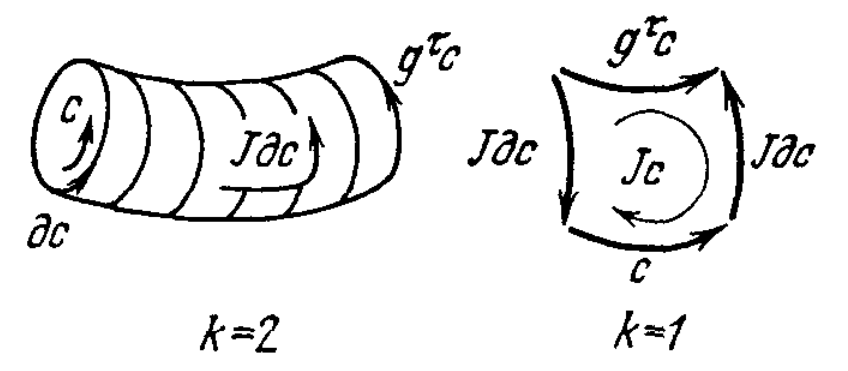
\includegraphics[width=0.3\textwidth]{imgs/chains.png}
    \caption{След цепи при гомотопии}
    \label{fig:сhains}
\end{figure}




\begin{to_thr}[]
    Гамильтонов фазовый поток сохраняет симплектическую структуру $(g^t)^* \omega^2 = \omega^2$. 
    \label{thrA1}
\end{to_thr}


\begin{to_lem}
    Пусть $\gamma$ -- 1-цепь в симплектическом многообразии $(M^{2n}, \omega^2)$. Пусть $g^t$  -- фазовый поток на $M$ с функцией Гамильтона $H$. Тогда
    \begin{equation*}
        \frac{d }{d \tau} \int_{J \gamma} \omega^2 = - \int_{g^\tau \gamma} d H.
    \end{equation*}
\end{to_lem}

\begin{proof}[$\triangle$]
Рассмотрим цепь $\gamma$ из одного куска $f \colon  [0, 1] \mapsto M$, пусть $f'(s, t) = g^t f(s)$, $\xi = \partial_s f'$ и $\eta = \partial_t f' \in TM_{f'(s, t)}$.

По определению интеграла
\begin{equation*}
    \int_{J\gamma} \omega^2 = \int_0^1 \int_0^\tau \omega^2 (\xi, \eta) \d t \d s
\end{equation*}
Но, по определению фазового потока $\eta$ -- вектор гамильтонова поля в точке $f'$, и снова по определению гамильтонова поля $\omega^2 (\eta, \xi) = \d H(\xi)$, тогда
\begin{equation*}
    \int_{J\gamma} \omega^2 = - \int_0^\tau \left(
        \int_{g^t \gamma}  \d H
    \right) \d \tau.
\end{equation*}
\end{proof}

Как некоторое следствие, можно выделить, что если $\gamma$ замкнута ($\partial \gamma =0$), то $\int_{J\gamma} \omega^2 = 0$, по теореме Стокса: $\int_\gamma \d H = \int_{\partial \gamma} H = 0$. 

\begin{proof}[$\triangle$оказательство теоремы]
    Рассмотрим некоторую 2-цепь, тогда для неё
    \begin{equation*}
        0 
        \overset{(1)}{=} 
        \int_{Jc} \d \omega^2 
        \overset{(2)}{=}
        \int_{\partial Jc} \omega^2 
        \overset{(3)}{=} 
        \int_{g^\tau c} - \int_c - \int_{J \partial c} \omega^2 
        \overset{(4)}{=} 
        \int_{g^\tau c}^{} \omega^2 - \int_c \omega^2,
    \end{equation*}
    где $(1)$ равенство верно по замкнутости $\omega^2$, второе по формуле Стокса, третье -- расписали границу цепи, и последнее по предыдущему следствию. 
\end{proof}

% \begin{equation*}
%     \frac{\partial^2 L}{\partial \dot{q}^i \dot{q}^j} = 
%     \frac{\partial p_j}{\partial \dot{q}^i},
%     \hspace{5 mm} 
%     \det\left(
%         \frac{\partial^2 L}{\partial \dot{q}^i \dot{q}^j} 
%     \right) = 0 = 
%     \det \left(
%         \frac{\partial p_j}{\partial \dot{q}^i}
%     \right)
% \end{equation*}



\begin{to_def}
    Дифференциальная $k$-форма $\omega$ называется \textit{интегральным инвариантом} отображения $g$, если интегралы $\omega$ по любой $k$-мерной цепи $c$ и по её образу при отображении $g$ одинаковы: $\int_{g[c]} \omega = \int_x \omega$. 
\end{to_def}



\begin{to_thr}[аналог thr \ref{thrA1}]
    Задающая симплектическую структуру форма $\omega^2$ является интегральным инвариантом гамильтонова фазового потока. 
\end{to_thr}


Также $(\omega^2)^2 = \omega^2 \wedge \omega^2$, и друге <<степени>> являются интегральными инвариантами фазового потока. 

\begin{to_def}
    Отображение $g \colon  \mathbb{R}^{2n} \mapsto \mathbb{R}^{2n}$ называется \textit{каноническим}, если оно имеет $\omega^2$ интегральным инвариантом. Каждая из форм $\omega^4$, $\omega^6$, ..., $\omega^{2n}$ является интегральным инвариантом всякого канонического отображения. Следовательно, при каноническом отображении сохраняется сумма ориентированных площадей проекций на координтные плоскости $(p_i,\, q^j)$. В частности, \textit{канонические отображения сохраняют объёмы}. 
\end{to_def}


\begin{to_def}
    Дифференциальная $k$-форма $\omega$ называется \textit{относительным интегральным инвариантом} отображения $g \colon  M \mapsto M$, если $\int_{gc} \omega = \int_c\omega$ для всякой \textit{замкнутой} $k$-цепи $c$. 
\end{to_def}


\begin{to_thr}[]
    Пусть $\omega$ -- относительный интегральный инвариант отображения $g$, тогда $d \omega$ -- абсолютный абсолютный интегральный инвариант $g$. 
\end{to_thr}

\begin{proof}[$\triangle$]
 Пусть $c$ это $k+1$-цепь, тогда
 \begin{equation*}
     \int_c d \omega = \int_{\partial c} \omega = \int_{g \partial c} \omega = \int_{g c} d \omega.
 \end{equation*}
\end{proof}



Например, каноническое отображение имеет относительный интегральный инвариант $\omega^1 = \vc{p} \d \vc{q} = p_i \d q^i$. 


\begin{to_thr}[закон сохранения энергии]
    Функция $H$ является первым интегралом гамильтонова фазового потока с функцией Гамильтона $H$. 
\end{to_thr}

\begin{proof}[$\triangle$]
Производная $H$ по направлению $\eta$ равна значению $\d H$ на $\eta$. Тогда, по определению
\begin{equation*}
    \d H (\eta) = \omega^2 (\eta,  I \d H) = \omega^2 (\eta, \eta) = 0.
\end{equation*}
\end{proof}



\subsubsection*{Алгебра Ли векторных полей}


\begin{to_def}
    \textit{Алгеброй Ли} называется линейной пространство $L$ вместе с билинейной кососимметричной операцией (\textit{коммутатором}) $L \times  L \mapsto L$, удовлетворяющей тождеству Якоби
    \begin{equation*}
        \left[[A, B], C\right] + \left[[B, C], A\right] + \left[C, A], B\right] = 0.
    \end{equation*}
\end{to_def}


Со всяким гладким полем на многообразии связаны следуюшие два объекта: \vspace{-2mm}
\begin{enumerate*}
    \item \textit{Однопараметрическая группа диффеоморфизмов}, или \textit{поток} $A^t \colon  M \mapsto M$, для которого $\vc{A}$ -- поле скоростей:
    $d_t |_{t=0} A^t (x) = \vc{A}(x)$.
    \item \textit{Производная по направленю} поля $\vc{A}$: дял всякой функции $\varphi M \mapsto \mathbb{R}$ \textit{производная по направлению} $\vc{A}$ есть $L_{\smallvc{A}} \varphi $ такая, что $(L_{\smallvc{A}}\varphi )(x) = d_t |_{t=0} \varphi(A^t x)$.
\end{enumerate*}


Вполне естественно ввести коммутатор дифференцирования по направлениям $\vc{A}$ и $\vc{B}$:
\begin{equation*}
    \frac{\partial^2}{\partial s \ \partial t} \bigg|_{t=s=0} \varphi(A^t B^s x) - \varphi(B^s A^t x) = \left(
        L_{\smallvc{B}} L_{\smallvc{A}} - L_{\smallvc{A}} L_{\smallvc{B}} \varphi
    \right) (x),
\end{equation*}
где возникший коммутатор -- дифференциальный оператор первого порядка, который соответсвует некотором векторному полю $\vc{C}$.


\begin{to_def}
    \textit{Скобкой Пуассона} или \textit{коммутатором} двух векторных полей $\vc{A}$ и $\vc{B}$ на многообразии $M$ называется векторное поле $C$, для которого
    \begin{equation*}
        \li{C} = \li{B} \li{A} - \li{A} \li{B}, \hspace{5 mm} \vc{C} = [\vc{A}, \vc{B}],
    \end{equation*}
    или, в компонентах:
    \begin{equation*}
        [\vc{A}, \vc{B}]^j = 
        B^i \partial_i A^j - A^i \partial_i B^j.
    \end{equation*}
\end{to_def} 

\begin{to_thr}[]
    Скобка Пуассона превращает линейное пространство векторных полей на многообразии $M$ в алгебру Ли, в частности  выполняется тождество Якоби. 
\end{to_thr}

\begin{to_thr}[]
    Два потока $A^t$ и $B^s$ коммутируют тогда и тоько тогда, когда скобка Пуассона соответсвующих векторных полей $[\vc{A}, \vc{B}]$ равна нулю. 
\end{to_thr}





\subsubsection*{Алгебра Ли функций Гамильтона}


Вернемся к симплектическому многообразию, функции $H \colon  M^{2n} \mapsto \mathbb{R}$ заданной на многообразие, и соответствующей однопараметрической группе $g_H^t \colon  M^{2n} \mapsto M^{2n}$ канонических преобразований, $M^{2n}$ -- фазовый поток с функцией гамильтона $H$. Пусть $F \colon  M^{2n} \mapsto \mathbb{R}$ -- другая функция на многообразии $M^{2n}$.

\begin{to_def}
    Скобкой Пуассона $\left\{F,\, H\right\}$ функций $F$ и $H$, заданных на симплектическом многообразии, называется производная функции $F$ по направлению фазового потока с функцией $H$:
    \begin{equation*}
        \{F, H\} (x) = \frac{d }{d t} \bigg|_{t=0} F(g^t_H (x)).
    \end{equation*}
\end{to_def}

\begin{to_con}
    Функция $F$ тогда и только тогда является первым интегралом фазового потка с функцией Гамильтона $H$, когда её скобка Пуассона с $H$ равна нулю: $\{F,\, H\} \equiv 0$.
\end{to_con}


Если вспомним про изоморфизм $I$ между 1-формами и векторными полями  вида $\omega^2 (\eta,\, I \omega^1) = \omega^1 (\eta)$. Вектор скорости фазового потока $g_H^t = I \d H$.

Скобка Пуассона функций $F$ и $H$ равна равна значению 1-формы $\d F$ на векторе $I \d H$ скорости фазового потка с функцией Гамильтона $H$:
\begin{equation*}
    \{F,\, H\} = \d F (I\d H) = 
    \omega^2(I \d H, I \d F),
\end{equation*}
откуда очевидно, что скобка Пуассона кососимметрическая билинейная функция. Тогда можем обобщить теорему Э. Нётер:

\begin{to_thr}[]
    Если функция Гамильтона $H$ выдерживает группу канонических преобразований, заданную гамильтонианом $F$, то $F$ есть первый интеграл системы с функцией Гамильтона $H$. 
\end{to_thr}

Стоит заметит, что в координатах $\{F,\, H\} = \left[
    I \d H,\, I \d F
\right] = \[\grad H,\, \grad F\] = \partial_{p_i} H \partial_{q^i} F - 
\partial_{q^i} H \partial_{p_i}F$. Также стоит вспомнить, что в базисе $(\vc{p},\, \vc{q})$ $I$ имеет вид 
\begin{equation*}
    \begin{pmatrix}
        0 & -E \\
        E & 0
    \end{pmatrix}.
\end{equation*}


% \secnum{7}{Инвариантные торы}
% 20, 21


% \secnum{8}{Теория возмущений} %+w9
% 22, 23, 24, 25


% \secnum{9}{Адиабатические и интегральные инварианты} %+w6
% 26, 27, 28


% \secnum{10}{ДинСистемы: хаос} %+ДинСистемы_1sem
% 29, 30


% \secnum{11}{Введение в КАМ-теорию} %+w10
% 31, 32, 33, 34
